\documentclass{standalone}
\usepackage{tikz}
\usetikzlibrary{patterns, positioning}

\begin{document}
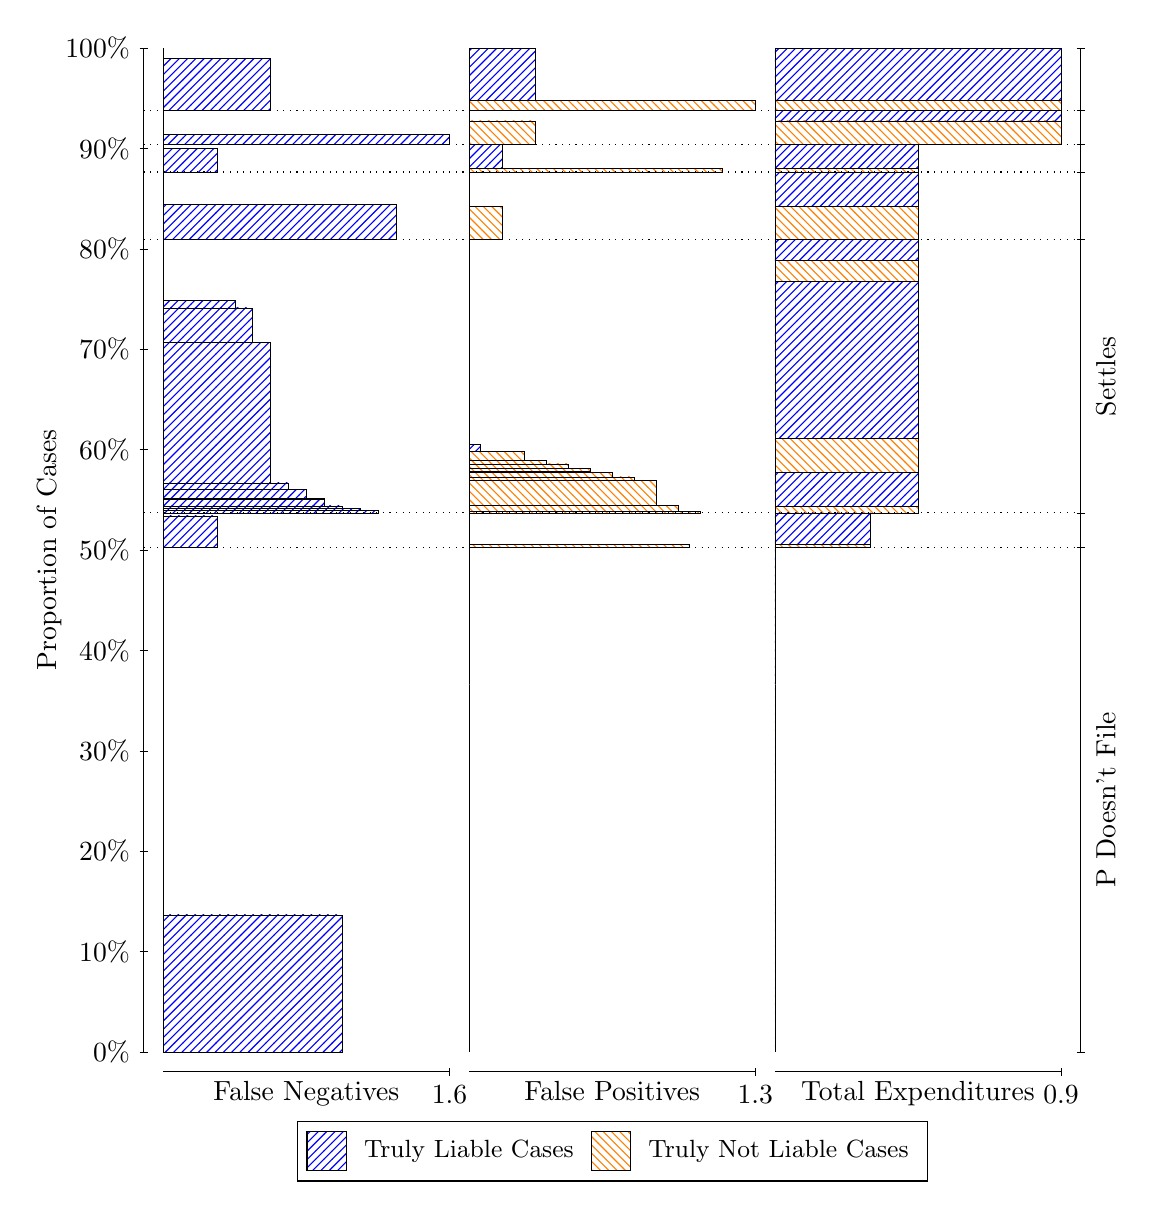
\begin{tikzpicture}
\draw[black, very thin] (1.5,1.75) -- (1.5,14.5);
\node[rotate=90, anchor=center] at (0.3, 8.125) {Proportion of Cases};
\draw[black, very thin] (1.45,1.75) -- (1.55,1.75);
\node[anchor=east] at (1.45, 1.75) {0\%};
\draw[black, very thin] (1.45,3.025) -- (1.55,3.025);
\node[anchor=east] at (1.45, 3.025) {10\%};
\draw[black, very thin] (1.45,4.3) -- (1.55,4.3);
\node[anchor=east] at (1.45, 4.3) {20\%};
\draw[black, very thin] (1.45,5.575) -- (1.55,5.575);
\node[anchor=east] at (1.45, 5.575) {30\%};
\draw[black, very thin] (1.45,6.85) -- (1.55,6.85);
\node[anchor=east] at (1.45, 6.85) {40\%};
\draw[black, very thin] (1.45,8.125) -- (1.55,8.125);
\node[anchor=east] at (1.45, 8.125) {50\%};
\draw[black, very thin] (1.45,9.4) -- (1.55,9.4);
\node[anchor=east] at (1.45, 9.4) {60\%};
\draw[black, very thin] (1.45,10.675) -- (1.55,10.675);
\node[anchor=east] at (1.45, 10.675) {70\%};
\draw[black, very thin] (1.45,11.95) -- (1.55,11.95);
\node[anchor=east] at (1.45, 11.95) {80\%};
\draw[black, very thin] (1.45,13.225) -- (1.55,13.225);
\node[anchor=east] at (1.45, 13.225) {90\%};
\draw[black, very thin] (1.45,14.5) -- (1.55,14.5);
\node[anchor=east] at (1.45, 14.5) {100\%};

\draw[black, very thin] (13.4,1.75) -- (13.4,14.5);
\draw[black, very thin] (13.35,1.75) -- (13.45,1.75);
\node[anchor=west] at (13.35, 1.75) {};
\draw[black, very thin] (13.35,8.1572) -- (13.45,8.1572);
\node[anchor=west] at (13.35, 8.1572) {};
\draw[black, very thin] (13.35,8.5959) -- (13.45,8.5959);
\node[anchor=west] at (13.35, 8.5959) {};
\draw[black, very thin] (13.35,12.07) -- (13.45,12.07);
\node[anchor=west] at (13.35, 12.07) {};
\draw[black, very thin] (13.35,12.925) -- (13.45,12.925);
\node[anchor=west] at (13.35, 12.925) {};
\draw[black, very thin] (13.35,13.273) -- (13.45,13.273);
\node[anchor=west] at (13.35, 13.273) {};
\draw[black, very thin] (13.35,13.704) -- (13.45,13.704);
\node[anchor=west] at (13.35, 13.704) {};
\draw[black, very thin] (13.35,14.5) -- (13.45,14.5);
\node[anchor=west] at (13.35, 14.5) {};

\draw[black, very thin, pattern color=blue, pattern=north east lines] (1.75,1.75) rectangle (4.0208,3.491);
\draw[black, very thin, pattern color=orange, pattern=north west lines] (1.75,3.491) rectangle (1.75,8.1572);
\draw[black, very thin, pattern color=blue, pattern=north east lines] (1.75,8.1572) rectangle (2.4312,8.5588);
\draw[black, very thin, pattern color=orange, pattern=north west lines] (1.75,8.5588) rectangle (1.75,8.5959);
\draw[black, very thin, pattern color=blue, pattern=north east lines] (1.75,8.5959) rectangle (4.475,8.6282);
\draw[black, very thin, pattern color=blue, pattern=north east lines] (1.75,8.6282) rectangle (4.2479,8.651);
\draw[black, very thin, pattern color=blue, pattern=north east lines] (1.75,8.651) rectangle (4.0208,8.6846);
\draw[black, very thin, pattern color=blue, pattern=north east lines] (1.75,8.6846) rectangle (3.7937,8.7677);
\draw[black, very thin, pattern color=blue, pattern=north east lines] (1.75,8.7677) rectangle (3.7937,8.7779);
\draw[black, very thin, pattern color=blue, pattern=north east lines] (1.75,8.7779) rectangle (3.5667,8.8907);
\draw[black, very thin, pattern color=blue, pattern=north east lines] (1.75,8.8907) rectangle (3.3396,8.9765);
\draw[black, very thin, pattern color=blue, pattern=north east lines] (1.75,8.9765) rectangle (3.1125,10.759);
\draw[black, very thin, pattern color=blue, pattern=north east lines] (1.75,10.759) rectangle (2.8854,11.199);
\draw[black, very thin, pattern color=blue, pattern=north east lines] (1.75,11.199) rectangle (2.6583,11.293);
\draw[black, very thin, pattern color=orange, pattern=north west lines] (1.75,11.293) rectangle (1.75,12.07);
\draw[black, very thin, pattern color=blue, pattern=north east lines] (1.75,12.07) rectangle (4.7021,12.51);
\draw[black, very thin, pattern color=orange, pattern=north west lines] (1.75,12.51) rectangle (1.75,12.925);
\draw[black, very thin, pattern color=blue, pattern=north east lines] (1.75,12.925) rectangle (2.4312,13.225);
\draw[black, very thin, pattern color=orange, pattern=north west lines] (1.75,13.225) rectangle (1.75,13.273);
\draw[black, very thin, pattern color=blue, pattern=north east lines] (1.75,13.273) rectangle (5.3833,13.402);
\draw[black, very thin, pattern color=orange, pattern=north west lines] (1.75,13.402) rectangle (1.75,13.704);
\draw[black, very thin, pattern color=blue, pattern=north east lines] (1.75,13.704) rectangle (3.1125,14.368);
\draw[black, very thin, pattern color=orange, pattern=north west lines] (1.75,14.368) rectangle (1.75,14.5);
\draw[black, very thin, pattern color=orange, pattern=north west lines] (5.6333,1.75) rectangle (5.6333,6.4162);
\draw[black, very thin, pattern color=blue, pattern=north east lines] (5.6333,6.4162) rectangle (5.6333,8.1572);
\draw[black, very thin, pattern color=orange, pattern=north west lines] (5.6333,8.1572) rectangle (8.4282,8.1943);
\draw[black, very thin, pattern color=blue, pattern=north east lines] (5.6333,8.1943) rectangle (5.6333,8.5959);
\draw[black, very thin, pattern color=orange, pattern=north west lines] (5.6333,8.5959) rectangle (8.5679,8.6148);
\draw[black, very thin, pattern color=orange, pattern=north west lines] (5.6333,8.6148) rectangle (8.2885,8.6928);
\draw[black, very thin, pattern color=orange, pattern=north west lines] (5.6333,8.6928) rectangle (8.009,9.011);
\draw[black, very thin, pattern color=orange, pattern=north west lines] (5.6333,9.011) rectangle (7.7295,9.0541);
\draw[black, very thin, pattern color=orange, pattern=north west lines] (5.6333,9.0541) rectangle (7.45,9.1156);
\draw[black, very thin, pattern color=orange, pattern=north west lines] (5.6333,9.1156) rectangle (7.1705,9.1218);
\draw[black, very thin, pattern color=orange, pattern=north west lines] (5.6333,9.1218) rectangle (7.1705,9.166);
\draw[black, very thin, pattern color=orange, pattern=north west lines] (5.6333,9.166) rectangle (6.891,9.2181);
\draw[black, very thin, pattern color=orange, pattern=north west lines] (5.6333,9.2181) rectangle (6.6115,9.2607);
\draw[black, very thin, pattern color=orange, pattern=north west lines] (5.6333,9.2607) rectangle (6.3321,9.3728);
\draw[black, very thin, pattern color=blue, pattern=north east lines] (5.6333,9.3728) rectangle (5.7731,9.4671);
\draw[black, very thin, pattern color=blue, pattern=north east lines] (5.6333,9.4671) rectangle (5.6333,12.07);
\draw[black, very thin, pattern color=orange, pattern=north west lines] (5.6333,12.07) rectangle (6.0526,12.484);
\draw[black, very thin, pattern color=blue, pattern=north east lines] (5.6333,12.484) rectangle (5.6333,12.925);
\draw[black, very thin, pattern color=orange, pattern=north west lines] (5.6333,12.925) rectangle (8.8474,12.972);
\draw[black, very thin, pattern color=blue, pattern=north east lines] (5.6333,12.972) rectangle (6.0526,13.273);
\draw[black, very thin, pattern color=orange, pattern=north west lines] (5.6333,13.273) rectangle (6.4718,13.574);
\draw[black, very thin, pattern color=blue, pattern=north east lines] (5.6333,13.574) rectangle (5.6333,13.704);
\draw[black, very thin, pattern color=orange, pattern=north west lines] (5.6333,13.704) rectangle (9.2667,13.835);
\draw[black, very thin, pattern color=blue, pattern=north east lines] (5.6333,13.835) rectangle (6.4718,14.5);
\draw[black, very thin, pattern color=orange, pattern=north west lines] (9.5167,1.75) rectangle (9.5167,6.4162);
\draw[black, very thin, pattern color=blue, pattern=north east lines] (9.5167,6.4162) rectangle (9.5167,8.1572);
\draw[black, very thin, pattern color=orange, pattern=north west lines] (9.5167,8.1572) rectangle (10.728,8.1943);
\draw[black, very thin, pattern color=blue, pattern=north east lines] (9.5167,8.1943) rectangle (10.728,8.5959);
\draw[black, very thin, pattern color=orange, pattern=north west lines] (9.5167,8.5959) rectangle (11.333,8.674);
\draw[black, very thin, pattern color=blue, pattern=north east lines] (9.5167,8.674) rectangle (11.333,9.1135);
\draw[black, very thin, pattern color=orange, pattern=north west lines] (9.5167,9.1135) rectangle (11.333,9.5425);
\draw[black, very thin, pattern color=blue, pattern=north east lines] (9.5167,9.5425) rectangle (11.333,11.534);
\draw[black, very thin, pattern color=orange, pattern=north west lines] (9.5167,11.534) rectangle (11.333,11.804);
\draw[black, very thin, pattern color=blue, pattern=north east lines] (9.5167,11.804) rectangle (11.333,12.07);
\draw[black, very thin, pattern color=orange, pattern=north west lines] (9.5167,12.07) rectangle (11.333,12.484);
\draw[black, very thin, pattern color=blue, pattern=north east lines] (9.5167,12.484) rectangle (11.333,12.925);
\draw[black, very thin, pattern color=orange, pattern=north west lines] (9.5167,12.925) rectangle (11.333,12.972);
\draw[black, very thin, pattern color=blue, pattern=north east lines] (9.5167,12.972) rectangle (11.333,13.273);
\draw[black, very thin, pattern color=orange, pattern=north west lines] (9.5167,13.273) rectangle (13.15,13.574);
\draw[black, very thin, pattern color=blue, pattern=north east lines] (9.5167,13.574) rectangle (13.15,13.704);
\draw[black, very thin, pattern color=orange, pattern=north west lines] (9.5167,13.704) rectangle (13.15,13.835);
\draw[black, very thin, pattern color=blue, pattern=north east lines] (9.5167,13.835) rectangle (13.15,14.5);
\draw[black, dotted] (1.5,8.1572) -- (13.4,8.1572);
\draw[black, dotted] (1.5,8.5959) -- (13.4,8.5959);
\draw[black, dotted] (1.5,12.07) -- (13.4,12.07);
\draw[black, dotted] (1.5,12.925) -- (13.4,12.925);
\draw[black, dotted] (1.5,13.273) -- (13.4,13.273);
\draw[black, dotted] (1.5,13.704) -- (13.4,13.704);
\draw[black, very thin] (1.75,1.5) -- (5.3833,1.5);
\node[anchor=north] at (3.5667, 1.5) {False Negatives};
\draw[black, very thin] (5.3833,1.45) -- (5.3833,1.55);
\node[anchor=north] at (5.3833, 1.45) {1.6};

\draw[black, very thin] (5.6333,1.5) -- (9.2667,1.5);
\node[anchor=north] at (7.45, 1.5) {False Positives};
\draw[black, very thin] (9.2667,1.45) -- (9.2667,1.55);
\node[anchor=north] at (9.2667, 1.45) {1.3};

\draw[black, very thin] (9.5167,1.5) -- (13.15,1.5);
\node[anchor=north] at (11.333, 1.5) {Total Expenditures};
\draw[black, very thin] (13.15,1.45) -- (13.15,1.55);
\node[anchor=north] at (13.15, 1.45) {0.9};

\node[black, centered, rotate=90] at (13.72, 4.9536) {P Doesn't File};

\node[black, centered, rotate=90] at (13.72, 10.333) {Settles};





\draw (7.449999999999999,1.5) node[draw=none] (baseCoordinate) {};
\begin{scope}[align=center]
        \matrix[scale=0.5, draw=black, below=0.5cm of baseCoordinate, nodes={draw}, column sep=0.1cm]{
            \node[rectangle, draw, minimum width=0.5cm, minimum height=0.5cm, pattern=north east lines, pattern color=blue] {}; &
            \node[draw=none, font=\small] (B) {Truly Liable Cases}; &
            \node[rectangle, draw, minimum width=0.5cm, minimum height=0.5cm, pattern=north west lines, pattern color=orange] {}; &
            \node[draw=none, font=\small] (B) {Truly Not Liable Cases}; \\
            };
\end{scope}

\end{tikzpicture}
\end{document}